%
% speziell.tex -- Spezielle Relativitätstheorie
%
% (c) 2017 Prof Dr Andreas Müller, Hochschule Rapperswil
%

\chapter{Spezielle Relativitätstheorie%
\label{skript:chapter:spezielle}}
\lhead{Spezielle Relativitätstheorie}
\rhead{}
Im neunzehnten Jahrhundert hat James Clark Maxwell die Theorien
über Elektriztität und Magnetismus zu einer einheitlichen Theorie
der Elektrodynamik zusammengefasst.
\index{Maxwell, James Clark}
\index{Elektrodynamik}
Diese Theorie ist die Grundlage aller Phänomene, mit denen sich
ein Elektroingenieur täglich herumschlägt.
Sie hat jedoch eine seltsame Eigenschaft, die schon sehr früh
aufgefallen ist.
Die Formeln der Mechanik von Galilei und Newton nicht ändern,
wenn man eine Koordinatentransformation der Form
\begin{equation}
\begin{aligned}
t'&=t\\
x'&=x+vt
\end{aligned}
\label{skript:kruemmung:galileitransformation}
\end{equation}
\index{Galiei-Transformation}
durchführt.
Diese Koordinatentransformation entspricht einer gleichförmigen
Bewegung des $(t',x')$-Koordinatensystems gegenüber dem 
$(t,x)$-Koordinatensystem.
Sie wird auch Galilei-Transformation genannt und wiederspiegelt die
Erfahrungstatsache, dass es in einem abfahrenden Zug schwierig ist
zu entscheiden, ob sich nun der Zug oder der Bahnhof in Bewegung setzt.

Die Gleichungen der Elektrodynamik verändern sich jedoch.
Es stellte sich daher die Frage, ob die Gleichungen der Elektrodynamik
nur einen Teilaspekt der Realität darstellen, oder ob die Gleichungen
der Mechanik nur eine Näherung sind, die für Geschwindigkeiten nahe
der Lichtgeschwindigkeiten nicht mehr zulässig sein würden.
Im letzten Fall wäre die
Galilei-Transformation~\eqref{skript:kruemmung:galileitransformation}
für solche Geschwidigkeiten auch nur eine Näherung, die durch
eine exaktere Formel ersetzt werden müsste, mit weitreichenden
Folgen für die Mechanik bei sehr hohen Geschwindigkeiten.

Es hat sich herausgestellt, dass tatsächlich die klassische Mechanik
angepasst werden muss.
Einstein hat diesen Schritt 1905 in seiner speziellen Relativitätstheorie
vollzogen.
Ziel dieses Abschnittes ist zu zeigen, welche Auswirkungen seine
Erkenntnis auf die Mechanik aber auch auf unser Weltbild hat.

\section{Lichtkegel}
\rhead{Lichtkegel}
Die Elektrodynamik sagt die Ausbreitungsgeschwindigkeit von
elektromagnetishen Wellen voraus.
Stellt man sich vor, dass elektromagnetische Wellen von einem
Medium geleitet werden, das man Äther nannte, dann müsste die
Geschwindigkeit von der Bewegung des Beobachters relativ zu
diesem Äther abhängen.
In hochgenauen Experimenten konnten Michelson und Morley und später
viele andere keine solche Abhängigkeit feststellen.
Dies steht zwar in Einklang mit der Theorie der Elektrodynamik,
wiederspricht der Galilei-Transformation, welche eine Veränderung
der Ausbreitungsgeschwindigkeit um $v$ vorhersagen würde.

Einstein hat die experimentell sehr gut bestätigte Konstanz der
Lichtgeschwindigkeit daher als Ausgangspunkt seiner Theorie genommen.
Entscheidend für die Physik ist, ob zwei Punkte sich mit elektromagnetischen
Wellen beeinflussen können.
Es ist daher nicht mehr ausreichend, nur Punkte miteinander zu vergleichen,
es muss auch immer die Zeit berücksichtigt werden, zu der sie verglichen
werden.
Raum und Zeit verschmelzen so zu einem einzigen vierdimensionalen
Kontinuum mit den Koordinaten $(t,x,y,z)$, welche wir die Raumzeit
nennen.
Quadrupel $(t,x,y,z)$ heissen auch {\em Ereignisse}.
\index{Ereignis}
Zwei Ereignisse $(t_1,x_1,y_1,z_1)$ und $(t_2,x_2,y_2,z_2)$ können
kausal voneinander abhängen, wenn ein Lichtsignal sich vom einen Ereignis
zum anderen Ereignis ausbreiten kann.
Dazu ist notwendig, dass der ``Abstand''
\begin{equation}
s^2
=
-c^2(t_1-t_2)^2
+
\mathstrut
\underbrace{
(x_1-x_2)^2
+
(y_1-y_2)^2
+
(z_1-z_2)^2}_{\text{Raumabstand}}
\label{skript:kruemmung:raumzeitabstand}
\end{equation}
gleich $0$ ist.
Breitet sich die Wirkung langsamer als mit Lichtgeschwindigket aus,
wird die zeitliche Differenz noch grösser sein, und damit der
Ausdruck~\eqref{skript:kruemmung:raumzeitabstand} negativ ist.

\begin{figure}
\centering
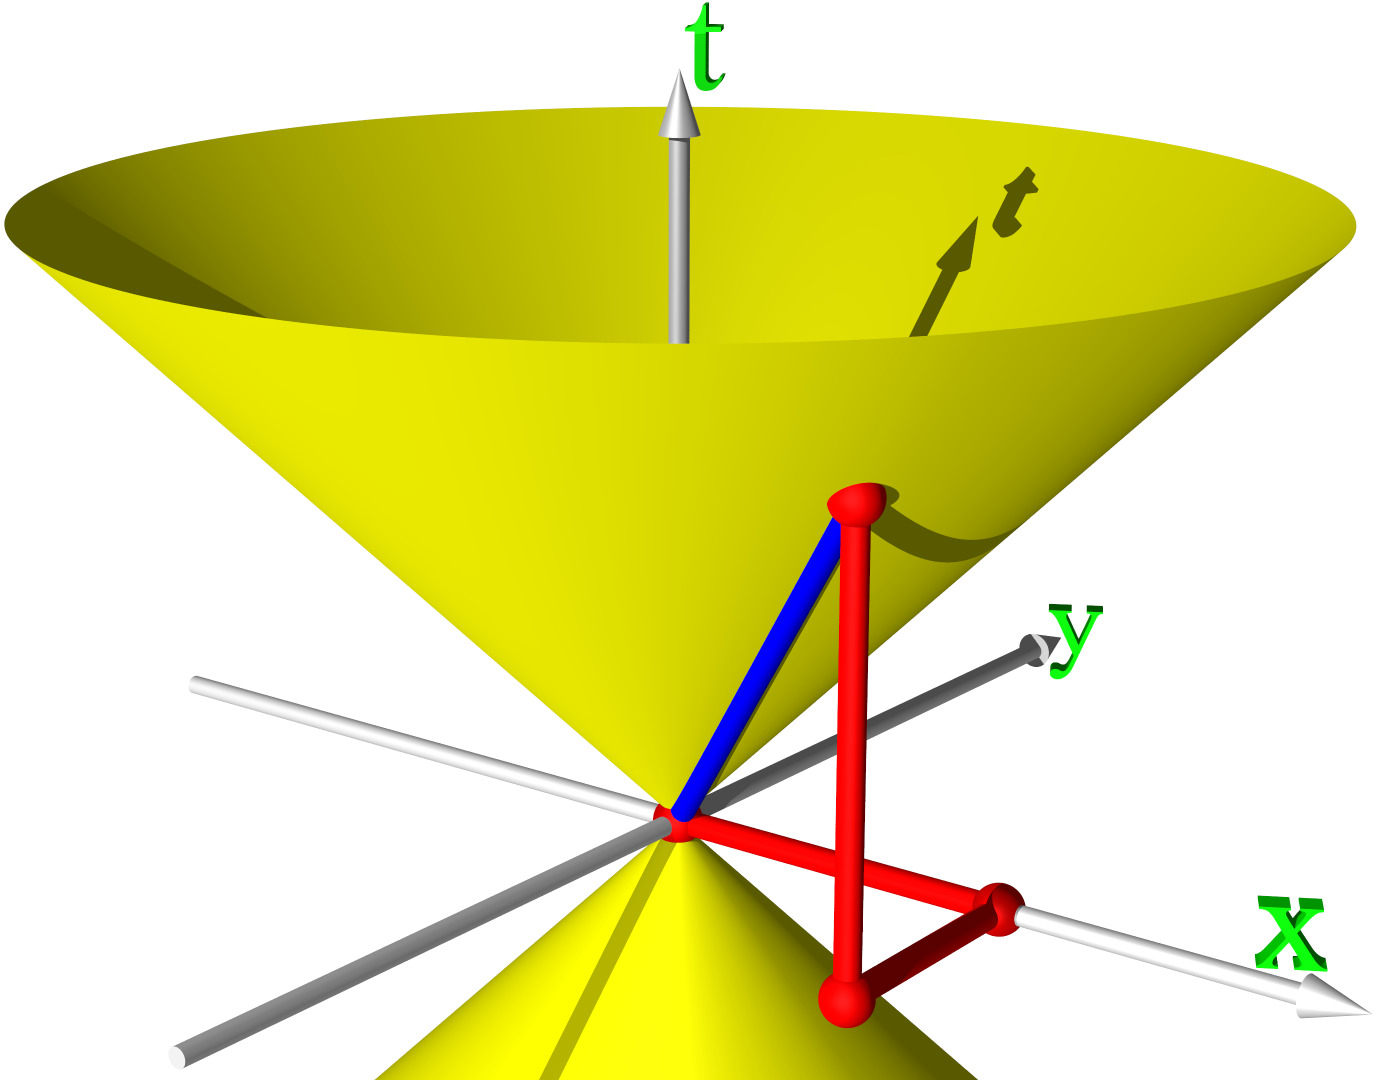
\includegraphics[width=\hsize]{chapters/3d/lichtkegel.jpg}
\caption{Lichtkegel ausgehend vom Nullpunkt zur Zeit $t=0$.
Alle Punkte innerhalb des Kegels mit $t>0$ liegen in der Zukunft des
Beobachters im Nullpunkt, solche mit $t<0$ in seiner Vergangenheit.
Punkte ausserhalb des Kegels können vom Nullpunkt aus nicht
beeinflusst werden.
Nur Punkte innerhalb des Kegels mit $t<0$ können Einfluss haben
auf den Nullpunkt.
\label{skript:kruemmung:fig:lichtkegel}}
\end{figure}

Das Vorzeichen des Ausdrucks~\eqref{skript:kruemmung:raumzeitabstand}
beschreibt also, ob zwei Ereignisse sich gegenseitig beeinflussen
können. 
Ist er negativ, dann ist eine Beeinflussung mit einer Wirkung möglich,
die sich weniger schnell als Licht ausbreitet.
Ist er gleich $0$, ist nur eine Beeinflussung mit einer Wirkung möglich,
die sich mit Lichtgeschwindigkeit ausbreitet.
Ist er positiv, ist keine gegenseitige Beeinflussung möglich.
Dies führt auf eine Unterteilung des Raumes in drei Gebiete
(Abbildung~\ref{skript:kruemmung:fig:lichtkegel}).
Die Fläche mit der Gleichung
\[
-c^2t^2+x^2+y^2+z^2=0
\]
heisst der Lichtkegel.
Ereignisse innerhalb des Lichtkegels mit $t>0$ können vom Nullpunkt aus
beeinflusst werden.
Ereignisse innerhalb des Lichtkegels imt $t<0$ können auf den Nullpunkt
Einfluss nehmen.
Alle anderen Ereignisse können den Nullpunkt weder beeinflussen
noch von ihm beeinflusst werden.
Sie müssen daher als die Gegenwart des Nullpunktes bezeichnet
werden.

Der Formalismus einer Metrik passt ganz hervorragend auf die hier
vorliegende Situation.
Verwenden wir als Koordinaten
\begin{align*}
x^0 &= ct,
&
x^1&=x,
&
x^2&=y,
&
x^3&=z,
\end{align*}
dann kann $s^2$ mit der Metrik
\begin{equation}
g_{\mu\nu}
=
\begin{pmatrix}
-1&0&0&0\\
 0&1&0&0\\
 0&0&1&0\\
 0&0&0&1
\end{pmatrix}
\label{skript:speziell:metrik}
\end{equation}
berechnet werden.
Die spezielle Relativitätstheorie beschreibt die Welt also einen
vierdimensionalen Raum, die Raum-Zeit, der Raumkoordinaten und Zeitkoordinate
in einem einzigen mathematischen Modell kombiniert.
Die Metrik~\eqref{skript:speziell:metrik} beschreibt dann die
Kausalitätsstruktur der Welt.

In diesem Bild gibt es also keinen sinnvollen Begriff der Gleichzeitigkeit
mehr.
Wäre das Universum nicht aus einem Punkt entstanden, wie das Big Bang-Modell
besagt, dann wäre bereits die Frage ``Wann ist das Universum entstanden''
unsinnig, denn es gibt keinen sinnvollen Art und Weise, wie etwas gleichzeitig
im ganzen Universum stattfinden könnte.
Diese Beobachtung hat zu Einsteins Zeit aber keine grossen Wellen
geworfen, denn die meisten Phyisker gingen davon aus, dass das Universum
ewig und statisch ist, dass es also gar keinen Anfang braucht.
Auch Einstein ging davon aus, was ihn später in seiner allgemeinene
Relativitätstheorie dazu gebracht hat, einen nicht weiter erklärbaren
Term hinzuzufügen, einzig um zu erreichen, dass das Universum statisch 
sein kann.

Wenn die Frage ``Wann ist das Universum entstanden'' überhaupt eine
sinnvolle Antwort haben soll, dann nur, wenn das Universum zur Zeit
der Entstehung nur ein Punkt gewesen ist.
Wenn das Universum ausgedehnt entstanden ist, dann ist die Frage
nach dem Entstehungszeitpunkt sinnlos.

\section{Lorentztransformation}
\rhead{Lorentztransformation}
Der Ausdruck~\eqref{skript:kruemmung:raumzeitabstand} ist nicht
invariant bei einer Galilei-Transformation.
Damit stellt sich die Frage, welche Transformationen denn
invariant wären.
Dies wären die Koordinaten-Änderungen, die zulässig sind, wenn
man das grundlegende Gesetz~\eqref{skript:kruemmung:raumzeitabstand}
der Kausalität erhalten will.

Zunächst sind Koordinatentransformationen, die nur die Raumkoordinaten
$x$, $y$ und $z$ beeinflussen, und den räumlichen Abstand nicht
ändern, zulässig.
Diese Transformationen sind aber wohlbekannt.
In der Linearen Algebra lernt man, dass genau die orthogonalen
Matrizen $A\in \textrm{O}(3)$, also Matrizen mit $A^tA=E$ diese
Eigenschaft haben.
Diese entsprechen räumlichen Drehungen und Spiegelungen.

Wenn sich aber zwei Koordinatensystem gegeneinander verschieben,
so wie bei der Galilei-Transformation, dann müssen auch die auch
die Zeitkoordinaten in die Transformation involviert sein.
Wir suchen also eine Koordinatentransformation, die nur die
$t$- und $x$-Koordinaten betrifft.
Wir können Sie in der Form
\begin{equation}
\begin{linsys}{3}
t'&=& a_{11}t&+&a_{12}x\\
x'&=& a_{21}t&+&a_{22}x
\end{linsys}
\end{equation}
ansetzen.
Wir verlangen jetzt aber, dass der
Ausdruck~\eqref{skript:kruemmung:raumzeitabstand}
unverändert bleibt.
Da die $y$- und $z$-Koordinaten ohnehin nicht involviert sind, bedeutet
das, dass
\begin{align*}
-c^2t^2 + x^2
&=
-c^2t'^2 + x'^2
\\
&=
-c^2(a_{11}t+a_{12}x)^2 + (a_{21}t+a_{22}x)^2
\\
&=
-c^2a_{11}^2t^2 -2c^2a_{11}a_{12}tx -c^2a_{12}^2x^2
+a_{21}^2t^2+2a_{21}a_{22}tx+a_{22}^2x^2
\\
&=
-(c^2a_{11}^2 - a_{21}^2)t^2
+2(-c^2a_{11}a_{12}+a_{21}a_{22})tx
+(-c^2a_{12}^2 + a_{22}^2)x^2.
\end{align*}
Da dies für beliebige Werte von $x$ und $t$ gelten muss, müssen die
Koeffizienten der beiden Seiten übereinstimmen. 
Wir erhalten damit für die Koeffizienten $a_{ik}$ die Gleichungen
\[
\begin{aligned}
c^2a_{11}^2-a_{21}^2&=c^2,
&&\Rightarrow&
a_{11}^2
-
\biggl(\frac{a_{21}}{c}\biggr)^2
&=1,
\\
-c^2a_{12}^2+a_{22}^2&=1,
&&\Rightarrow
&
a_{22}^2 - (ca_{12})^2&=1,
\\
a_{21}a_{22}&=c^2a_{11}a_{12}.
\end{aligned}
\]
Da die Differenz der Quadrate jeweils $1$ ist, können die Basen
als Werte des hyperbolischen Kosinus und Sinus dargestellt werden:
\[
\begin{aligned}
a_{11}&=\cosh\beta, &&&\frac{a_{21}}{c}&=\sinh\beta,
\\
a_{22}&=\cosh\gamma,&&&ca_{12}&=\sinh\gamma.
\end{aligned}
\]
Die dritte Gleichung lautet dann
\begin{align*}
a_{21}a_{22}=c\sinh\beta\cosh\gamma
&=
c^2a_{11}a_{12}=c^2\cosh\beta\frac1c\sinh\gamma
\\
c\sinh\beta\cosh\gamma
&=
c\cosh\beta\sinh\gamma
\\
\tanh\beta&=\tanh\gamma,
\end{align*}
es folgt $\beta=\gamma$.
Damit haben wir die gesuchte Transformation gefunden, es ist
\begin{equation}
\begin{pmatrix}
a_{11}&a_{12}\\
a_{21}&a_{22}
\end{pmatrix}
=
\begin{pmatrix}
 \cosh\beta&\frac1c\sinh\beta\\
c\sinh\beta&\cosh\beta
\end{pmatrix}
\end{equation}
Um die physikalische Bedeutung des Parameters $\beta$ zu verstehen, 
betrachten wir die Punkte $x=0$ für beliebige $t$.
Sie werten abgebildet auf
\[
x' = c\sinh\beta t
\]
Im $(t',x')$-Koordinatensystem bewegt sich also der Nullpunkt des 
$(t,x)$-Koordinatensystems mit der Geschwindigkeit
\[
v=c\sinh\beta.
\]
Der zugehörige Wert von $\cosh \beta$ ist
\[
\cosh^2\beta - \sinh^2\beta = 1
\qquad \Rightarrow \qquad
\cosh^2\beta = 1+\sinh^2\beta
\qquad \Rightarrow \qquad
\cosh\beta = \sqrt{1+\biggl(\frac{v}{c}\biggr)^2}.
\]
Der Parameter $\sinh\beta$ hat also die Bedeutung einer in Einheiten
der Lichtgeschwindigkeit gemessenen Geschwindigkeit.
Da also $v/c=\sinh\beta$ ist, kann man die Transformation auch
als
\begin{equation}
\begin{pmatrix}
a_{11}&a_{12}\\
a_{21}&a_{22}
\end{pmatrix}
=
\begin{pmatrix}
\displaystyle\sqrt{1+\biggl(\frac{v}{c}\biggr)^2}
	&\displaystyle\frac{v}{c^2} \\
v
	&\displaystyle\sqrt{1+\biggl(\frac{v}{c}\biggr)^2}
\end{pmatrix}
\label{skript:kruemmung:lorentz}
\end{equation}
schreiben.
Die Transformation 
\eqref{skript:kruemmung:lorentz}
heisst {\em Lorentz-Transformation}.
\index{Lorentz-Transformation}

Befindet sich ein Beobachter im ursprünglichen $t$-$x$-System in Ruhe
im Nullpunkt, dann ist seine Zeitkoordinate im $t'$-$x'$-System
\begin{equation}
t'=t\sqrt{1+\biggl(\frac{v}{c}\biggr)^2},
\label{skript:speziell:zeitdilatation}
\end{equation}
der Lauf der Zeit ist in den beiden Koordinatensystemen verschieden.
Im $t'$-$x'$-Koordinatensystem läuft die Zeit um den Faktor
\eqref{skript:speziell:zeitdilatation} gedehnt.

Die Darstellung \eqref{skript:kruemmung:lorentz} der Lorenztransformation
ist nicht sehr symmetrisch.
Dies liegt daran, dass die Zeit-Koordinate eine ganz andere Masseinheit
verwendet.
Schreibt man für die Koordinaten 
\[
\begin{aligned}
x^0&=ct,&
x^1&=x,&
x^2&=y,&
x^3&=z&
\end{aligned}
\]
dann wird die Lorentztransformation
\begin{equation}
\begin{pmatrix}
x^{0\prime}\\
x^{1\prime}\\
x^{2\prime}\\
x^{3\prime}
\end{pmatrix}
=
\begin{pmatrix}
\sqrt{1+\biggl(\displaystyle\frac{v}{c}\biggr)^2} & \displaystyle\frac{v}{c} & 0 & 0 \\
\displaystyle\frac{v}{c} & \sqrt{1+\biggl(\displaystyle\frac{v}{c}\biggr)^2} & 0 & 0 \\
      0     &                                      & 1 & 0 \\
      0     &                                      & 0 & 1 
\end{pmatrix}
\begin{pmatrix}
x^0\\x^1\\x^2\\x^3
\end{pmatrix}.
\label{skript:speziell:4lorentz}
\end{equation}
In dieser Form ist die Lorentztransformation klar symmetrischer.

\section{Weltlinien und Eigenzeit}
\rhead{Weltlinien und Eigenzeit}
Die Bewegung eines Teilchens in der Raum-Zeit ist eine Kurve
$(t(\tau), x(\tau), y(\tau), z(\tau)$
mit dem Parameter $\tau$, die man auch {\em Weltlinie} nennt.
\index{Weltlinie}
Da sich das Teilchen nicht mit Lichtgeschwindigkeit bewegen kann, muss
\[
-c^2t'(\tau)^2
+ x'(\tau)^2 + y'(\tau)^2 + z'(\tau)^2
<
0
\]
gelten, darin bezeichnet der Apostroph die Ableitung nach dem 
Parameter $\tau$.
Offenbar bewegt sich das Teilchen mit der Geschwindigkeit
\[
v^2 = \frac{x'(\tau)^2 + y'(\tau)^2 + z'(\tau)^2}{t'(\tau)^2}
\]
durch die Raumzeit.
Da sich das Teilchen bewegt, läuft die Zeit in einem Koordinatensystem,
das sich mit dem Teilchen mitbewegt, um den Faktor
\eqref{skript:speziell:zeitdilatation}
langsam.
Setzt man die Definitionen ein, erhält man
\begin{align*}
\sqrt{1+\frac{v^2}{c^2}}
&=
\sqrt{1+ \frac{x'(\tau)^2 + y'(\tau)^2 + z'(\tau)^2}{c^2t'(\tau)^2}}
\\
&=
-
\sqrt{-c^2t'(\tau)^2+x'(\tau)^2 + y'(\tau)^2 + z'(\tau)^2}\frac{1}{ct'(\tau)}
\end{align*}
Die im bewegten Koordinatensystem gemessene Zeit ist
\begin{align*}
\int
\sqrt{1+\frac{v^2}{c^2}}\,dt
&=
\sqrt{-c^2t'(\tau)^2+x'(\tau)^2 + y'(\tau)^2 + z'(\tau)^2}\frac{1}{ct'(\tau)}
\,dt
\\
&=
\int
\sqrt{-c^2t'(\tau)^2+x'(\tau)^2 + y'(\tau)^2 + z'(\tau)^2}\frac{1}{ct'(\tau)}
t'(\tau)\,d\tau
\\
&=
\int
\frac1c
\sqrt{-c^2t'(\tau)^2+x'(\tau)^2 + y'(\tau)^2 + z'(\tau)^2}
\,d\tau
\end{align*}
In $x^\mu$-Koordinaten bedeutet dies, dass
\begin{equation}
\int
\sqrt{1-\frac{v^2}{c^2}}\,dt
=
\int \frac1{c}\sqrt{-g_{\mu\nu}\dot x^\mu(\tau) \dot x^\nu(\tau)}\,d\tau
\label{skript:speziell:eigenzeit}
\end{equation}
die Zeit ist, die entlang der Kurve $x^\mu(\tau)$ für den
mitbewegten Beobachter vergangen ist.
Man nennt~\eqref{skript:speziell:eigenzeit} die {\em Eigenzeit} des
Beobachters, der sich entlang der Weltlinie $x^\mu(\tau)$ bewegt.
\index{Eigenzeit}

\section{Energie und Impuls}
\rhead{Energie und Impuls}
Ein Teilchen der Masse $m$, die im Nullpunkt ruht, hat keinen
Impuls.
In einem anderen Koordinatensystem nimmt hat das Teilchen dagegen
eine Geschwindigkeit, und damit auch einen Impuls.
Dies zeigt, dass eine koordinatensystemunabhägngige Beschreibung
nicht nur mit dem Impuls funktionieren kann.
Wir brauchen eine erweiterte Erhaltungsgrösse, die wir zur Beschreibung
der Bewegung eines Teilchens verwenden können.

Die Kurve $x^\mu(\tau)$ und die Ableitung nach dem Kurvenparameter sind
offenbar keine geeigneten Grössen, denn der Kurvenparameter ist
keine vom Koordinatensystem unabhängige Grösse.
Die Eigenzeit ist aber eine solche koordinatensystemunabhängige
Grösse, wir schliessen daraus, dass die Ableitung der Position
nach der Eigenzeit, die sogenannte Vierergeschwindigket, der einzig
sinnvolle Ersatz für die Geschwindigkeit.

Ein ruhendes Teilchen hat die Weltlinie
\[
t\mapsto (t, x, y, z)=(t,0,0,0),
\]
der Parameter ist die Koordinatenzeit.
Da das Teilchen keine Geschwindigkeit hat, ist $t$ auch die Eigenzeit,
und die Vierergeschwdingkeit $u^\mu$ ist der Vektor.
\[
\begin{aligned}
u^0 &= c
&
u^1&=u^2=u^3 = 0
\end{aligned}
\]
Seine Länge gemessen mit der Metrik ist
\[
g_{\mu\nu}u^\mu u^\nu=-c^2,
\]
sie ist eine koordinatensystemunabhängige Grösse.

Wendet man darauf eine Lorentztransformation mit Geschwindigkeit $v$ an,
erhält man den Vektor
\[
\begin{aligned}
u^0
&=
c\sqrt{1+\biggl(\frac{v}{c}\biggr)^2},
&
u^1
&=
\frac{v}{c}c
&&\text{und}
&
u^2&=u^3=0.
\end{aligned}
\]
Wir rechnen das Skalarprodukt mit Hilfe der Metrik nach:
\[
-(u^0)^2 + (u^1)^2 + (u^2)^2 + (u^3)^2
=
-c^2\biggl(1+\biggl(\frac{v}{c}\biggr)^2\biggr) + \frac{v^2}{c^2} c^2
=
-c^2 - v^2  + v^2
= 
-c^2.
\]







